\documentclass[11pt]{article}

\usepackage{times}
\usepackage[english]{babel}

% -----------------------------------------------
% especially use this for you code
% -----------------------------------------------

\usepackage{courier}
\usepackage{listings}
\usepackage{color}
\usepackage{tabularx}
\usepackage{graphicx}

\definecolor{Gray}{gray}{0.95}

\definecolor{mygreen}{rgb}{0,0.6,0}
\definecolor{mygray}{rgb}{0.5,0.5,0.5}
\definecolor{mymauve}{rgb}{0.58,0,0.82}

\lstset{language=C++,
	basicstyle = \normalsize\ttfamily,   % the size and fonts that are used
	tabsize = 2,                    % sets default tabsize
	breaklines = true,              % sets automatic line breaking
	keywordstyle=\color{blue}\ttfamily,
	stringstyle=\color{red}\ttfamily,
	commentstyle=\color{mygreen}\ttfamily,
	numbers=left,
	keepspaces=true,
	showspaces=false,
	showstringspaces=false,
}

\begin{document}

\title{Programming in C/C++ \\
       Exercises set seven: Allocation in Classes
}
\date{\today}
\author{Christiaan Steenkist \\
Diego Ribas Gomes \\
Jaime Betancor Valado \\
Remco Bos \\
}

\maketitle

\section*{Assignment 58, \texttt{Strings} as a value-class}
We implemented the copy and move constructor as well as the assignment operator.

\subsection*{Code listings}
\lstinputlisting[caption = strings.h]{src/a58/strings/strings.h}
\lstinputlisting[caption = Copy constructor]{src/a58/strings/copyconstr.cc}
\lstinputlisting[caption = Move constructor]{src/a58/strings/moveconstr.cc}
\lstinputlisting[caption = Assignment operator]{src/a58/strings/operator=.cc}
\lstinputlisting[caption = swap.cc]{src/a58/strings/swap.cc}

\section*{Assignment 59, swapping}
Here we answer some questions about swapping.

\subsection*{Example code}
\begin{lstlisting}
void Class::swap(Class &other)
{
	char buffer[sizeof(Class)];
	memcpy(buffer,  this,   sizeof(Class)); //Operation 1
	memcpy(this, &other, sizeof(Class));  //Operation 2
	memcpy(&other, buffer,  sizeof(Class)); //Operation 3	
}
\end{lstlisting}

\subsection*{Explanation}
\begin{figure}[!ht]
\caption{A before-after diagram}
\centering
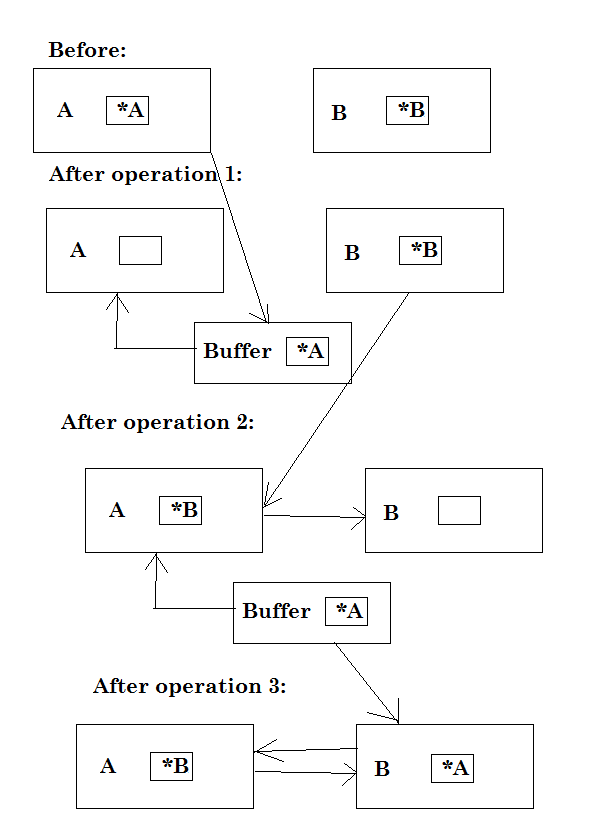
\includegraphics[width=0.5\textwidth]{src/a59/a59.png}
\end{figure}

Before the fast swap is done, an object A has a pointer data member *A to itself and an object B has a pointer data member *B to itself.
Pointers are variables that hold a memory address (in this case its current object).
The pointers keep pointing to the memory address they were defined for.
After operation 1, the pointer *A is moved to the buffer, but still points to its previous current object A.
After operation 2, the pointer *B is moved to object A, but still points to its previous current object B.
After operation 3, the pointer *A is moved to object B, and is still pointing to object A.
This results in a situation where the objects have swapped data members, however they now point to each other.
So the self-pointing property of the class is gone.

Using the keyword 'this' prevents this situation.
The 'this' keyword is placed in front of the data member and then points to the current object where the data member resides.
After doing the swapping like above but with the 'this' keyword, the data members of A and B are swapped. They still have the 'this' keyword
in front of them and now it still a self-pointing class. 

\section*{Assignment 60, the default keyword}
In the example of slide 30, 'default' wasn't specified for the copy constructor because it would defeat the purpose of explicitly defining it, which is to prevent wild pointers. In that case, the trivial copy constructor would be used, copying struct- or class- objects member-wise and, considering that the class allocates memmory for its own use, resulting in wild pointers.

One case where specifying default for a copy constructor could make sense would be for a class that simultaneously:
\begin{enumerate}
\item does NOT have pointer data members pointing at its own data and
\item have had its copy constructor suppressed by declarations of either the move constructor or the move assignment operator.
\end{enumerate}
Another would be to default the copy constructor in the header file as a form of documentation, to make it clear for the users.

\section*{Assignment 61, copy elision}
Here we show some situations where copy elision is and isn't used. First we are asked to define a class Demo:
\lstinputlisting[caption = Demo.h]{src/a61/Demo.h}
Also, we are asked to implement a Demo function in which:
\subsection*{Copy elision is used}
\lstinputlisting[caption = Copy Elision.cc]{src/a61/copy_elision.cc}
\subsection*{Move constructor is used}
\lstinputlisting[caption = Move constructor.cc]{src/a61/move_construct.cc}
\subsection*{Copy assignment is used}
\lstinputlisting[caption = Copy assignment.cc]{src/a61/copy_assignment.cc}
\subsection*{Move assignment is used}
\lstinputlisting[caption = Move assignment.cc]{src/a61/move_assignment.cc}


\section*{Assignment 62}
We have constructed a \texttt{Matrix} class that can handle any size matrix according to the specifications of the assignment.
All requested functions have been implemented and an example main function has been made showing off valid and invalid uses.

\subsection*{Matrix class}
\lstinputlisting[caption = matrix.ih]{src/a62/matrix/matrix.ih}
\lstinputlisting[caption = matrix.h]{src/a62/matrix/matrix.h}
\lstinputlisting[caption = copyconstructor.cc]{src/a62/matrix/copyconstructor.cc}
\lstinputlisting[caption = destructor.cc]{src/a62/matrix/destructor.cc}
\lstinputlisting[caption = identity.cc]{src/a62/matrix/identity.cc}
\lstinputlisting[caption = matrix1.cc]{src/a62/matrix/matrix1.cc}
\lstinputlisting[caption = matrix2.cc]{src/a62/matrix/matrix2.cc}
\lstinputlisting[caption = moveconstructor.cc]{src/a62/matrix/moveconstructor.cc}
\lstinputlisting[caption = moveoperator=.cc]{src/a62/matrix/moveoperator=.cc}
\lstinputlisting[caption = ncols.cc]{src/a62/matrix/ncols.cc}
\lstinputlisting[caption = nrows.cc]{src/a62/matrix/nrows.cc}
\lstinputlisting[caption = operator=.cc]{src/a62/matrix/operator=.cc}
\lstinputlisting[caption = row.cc]{src/a62/matrix/row.cc}
\lstinputlisting[caption = swap.cc]{src/a62/matrix/swap.cc}
\lstinputlisting[caption = tr.cc]{src/a62/matrix/tr.cc}

\subsection*{Main}
\lstinputlisting[caption = main.ih]{src/a62/main.ih}
\lstinputlisting[caption = main.h]{src/a62/main.h}
\lstinputlisting[caption = main.cc]{src/a62/main.cc}
\lstinputlisting[caption = printmatrix.cc]{src/a62/printmatrix.cc}

\end{document}
